\section{RESULTS}

The selection of an IPC method for robotics must be done on a case by case basis by evaluating the design goals and intended implementation. Each of the IPCs discussed in this paper offer strengths and weaknesses that the designer will need to accommodate. Code portability, data integrity, message latency, and system architecture all play an essential role in the selection process. While standardizing a communication protocol for the entire system may make implementation easier at the onset of a project, additional effort to optimize the system at a link by link level will vastly improve the operation of the robot. The results of the testing and research done in this paper conclude that combining different IPC methods within a robotic system allow for optimal message latency and flexibility of the system.

The ACH messaging system provides the ideal combination of speed and flexibility and should be utilized for internal messaging within a contiguous set of hardware. With the ability to configure an ACH channel as either blocking or non-blocking, the system can perform synchronously or asynchronously depending on the needs for the data. Additional configuration options allow the channel to be set as a FIFO or LIFO buffer without overwriting or losing any message data. The robot can access and react to the most recent sensor data while continuously logging the all data as it arrives. The synchronization provided internally by the data channels abstract the more complicated programming locks and allow for easily implemented, thread safe operation on multicore robots. As multicore embedded SBCs become increasingly available, ACH's synchronization allows for portability and upgradeable between single and multicore systems.

The use of sockets is recommended for all network communication to and from the robot. Sockets is a standard POSIX library and its use allows for modular addition of sensors, controllers, and other networked systems. Robots often operate in a real time environment and message latency is of critical importance. UDP excels at fast one directional communication. Data packets can be designed to be small in size to reduce, if not eliminate, any issues of dropped messages. Additionally, the data rate can be increased to the point where any missed message are made irrelevant by new data before the robot would notice. For situations where minimizing latency is a primary design goal and missed messages can be accepted then UDP is the recommended IPC. Figure \ref{fig:idealsystem} below details how an ideal system should be designed for minimal latency.

\begin{figure*}[t]
 \centering
 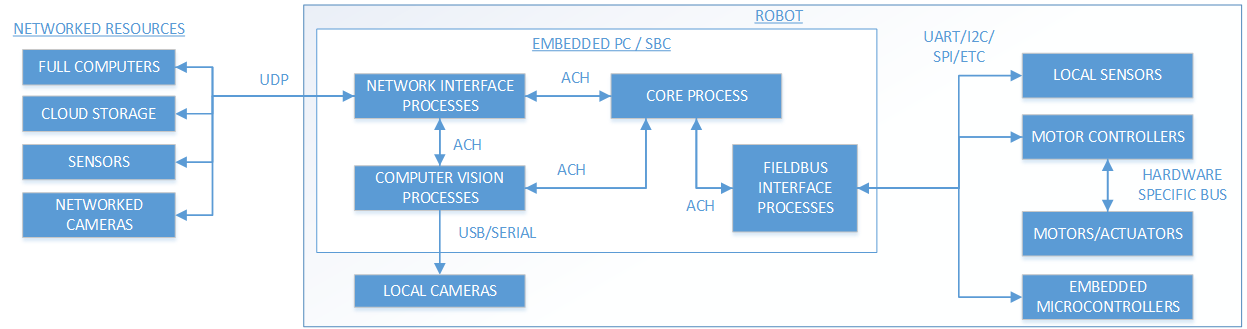
\includegraphics[width=2.0\columnwidth]{./images/idealsystem.png}
  \caption{Ideal System: Minimal Latency. This diagram shows how UDP and ACH IPC methods should be used for relevant system components.}
  \label{fig:idealsystem}
\end{figure*}

  Processing the large amount of messages into an ACH channel is critical to ensure usability of this method. This eliminates the issues of lost messages after the sockets buffer fills and prevents data obsolescence that would occur from a robot receiving data faster than it can process it. This method can be used with both UDP and TCP. The implementation of TCP is recommended with data integrity is of critical importance. For an ideal system that favors complete data transmission over increased latency then TCP should be utilized in conjunction with ACH. Figure \ref{fig:idealsystemtcp} details how an ideal system should be designed for data integrity.

\begin{figure*}[tbhp]
 \centering
 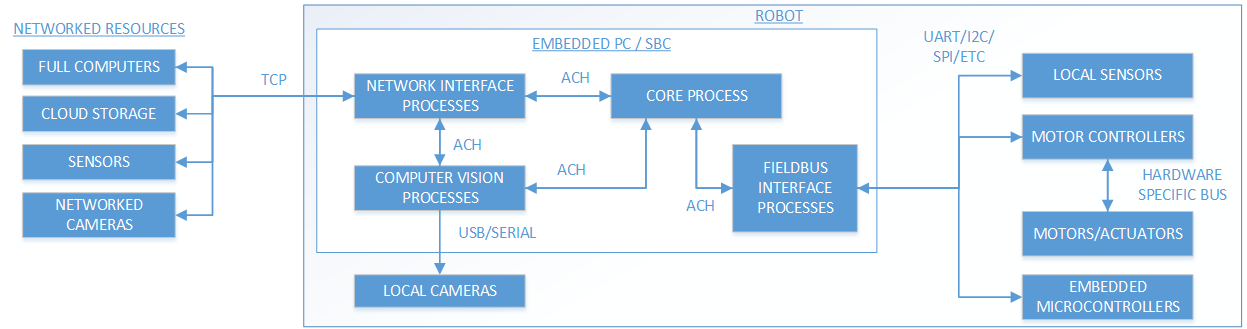
\includegraphics[width=2.0\columnwidth]{./images/idealsystem_integrity.png}
  \caption{Ideal System: Data Integrity. This diagram shows how TCP and ACH IPC methods should be used for relevant system components.}
  \label{fig:idealsystemtcp}
\end{figure*} 

The remaining IPC methods discussed in this paper should be used if a specific requirement dictates a specialized approach. The latency of a ZeroMQ message is detrimental to the real time operation of a robot. The only situation in which ZeroMQ should be implemented is when the system being designed requires a complex topology of processes that need to adhere to a publish/subscribe protocol. Robots are usually developed with a central command process that communicates with sub-processes, thus eliminating the advantages of ZeroMQ. 

ROS provides a vast library of modules to draw on for implementing hardware into the system. It is open source and supported on a wide variety of platforms. This reduces the amount of low level coding that needs to be written for each piece of hardware. This is advantageous for quickly building a system and reducing the amount of effort at the programming level. It fails to provide any real time support and the message latency and the head of line blocking nature of its TCP based messaging is problematic for high data transmission rates. ROS excels at building existing hardware and robotics into a viable system, but is not an ideal candidate for a custom built application.

While every robot is implemented differently, a combination of ACH channels and UDP/TCP sockets will be a viable application for the majority of systems. The flexibility and speed of the combined communication methods create a robust and modular link for real time robots to both internal and external components. 
